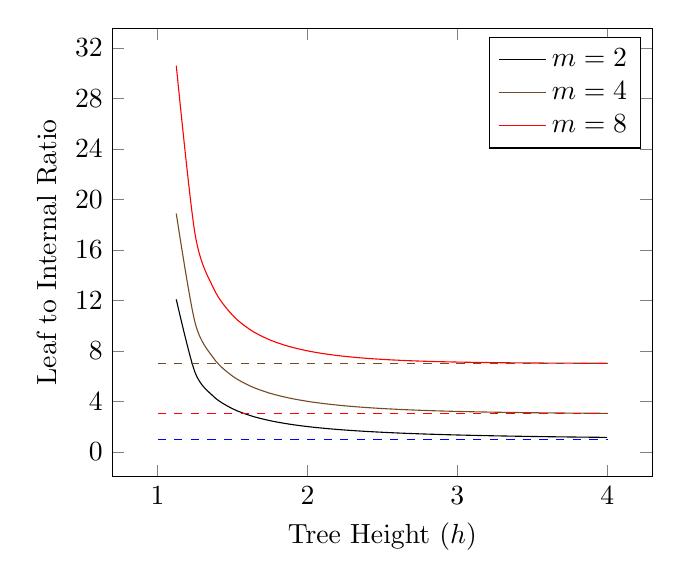
\begin{tikzpicture}
	\begin{axis}
		[
			xlabel={Tree Height ($h$)},
			ylabel={Leaf to Internal Ratio},
			xtick distance=1,
			ytick distance=4,
			domain=1:4,
			smooth
		]
		\pgfplotsinvokeforeach{2,4,8} {
			\addplot+[cycle list name=color list, mark=none]
				{(1-#1) / (#1^(1-x) - 1)};
			\addlegendentry{$m=#1$}
		}
		\pgfplotsset{cycle list shift=-3}
		\pgfplotsinvokeforeach{2,4,8} {
			\addplot+[cycle list name=color list, mark=none, dashed] {#1-1};
		}
	\end{axis}
\end{tikzpicture}
